\documentclass[a4paper,12pt]{article}
\usepackage[utf8]{inputenc}
\usepackage[ngerman]{babel}
\usepackage{graphicx}
\usepackage{svg}
\usepackage{booktabs}
\usepackage{array}
\usepackage{geometry}
\usepackage{hyperref}
\hypersetup{breaklinks=true}
\usepackage{caption}
\usepackage{subcaption}
\usepackage{hyphenat}
\usepackage{amsmath}
\usepackage{titlesec} % Para evitar títulos al final de una página
\usepackage{enumitem} % Para listas compactas
\usepackage{float} % Para controlar la ubicación de figuras y tablas
\usepackage{tabularx} % Asegúrate de incluir esto en el preámbulo
\usepackage{booktabs} % Mejora el diseño de las tablas
\usepackage{array} % Mejora la alineación de las columnas
\usepackage{graphicx} % Permite redimensionar tablas si es necesario
\usepackage{makecell} % Permite escribir encabezados en múltiples líneas

\geometry{a4paper, margin=1in}

\begin{document}

\begin{titlepage}
    \centering
    \includesvg[width=0.3\textwidth]{images/HFU_logo.svg}\\[0.5cm]
    {\Huge \textbf{Protokoll}}\\[0.2cm]
    {\LARGE Labor 2: Verbesserung der Adh\"asion durch Plasmabehandlung}\\[1cm]

    \vfill
    \vspace{12cm}
    \textbf{Autoren:}\\
    Adam Rshwany(277264), Markus Abrell(277261), Manuel Caipo(286577), Selina Sivac(277488)\\[0.3cm]

    \textbf{Studiengang:}\\
    Advanced Precision Engineering (M.Sc.)\\[0.3cm]

    \textbf{Hochschule Furtwangen}\\
    Wintersemester 2024/2025\\[0.3cm]

    \vfill
    \date{\today}
\end{titlepage}

\section{Einleitung}

Viele Polymere zeichnen sich durch eine geringe Oberflächenspannung aus, 
wodurch das Applizieren von Klebstoffen erschwert wird. Um die 
Oberflächenspannung zu erhöhen oder die Oberfläche zu reinigen, können 
diese mit Plasma behandelt werden \cite{ref1, ref2}. Je nach 
Werkstoffanforderungen können unterschiedliche Plasmabehandlungen zum 
Einsatz kommen. Eine solche Methode ist die Aktivierung durch 
Atmosphärenplasma.

Beim Atmosphärenplasma wird das Gas bei atmosphärischem Druck durch 
elektrische Entladung ionisiert. Die Ionisierung hat zur Folge, dass 
die reaktiven Teilchen die Verunreinigungen auf dem Substrat entfernen.
 Alternativ können die Ionen die chemischen Strukturen der Ablagerungen 
 fragmentieren. Bei der Fragmentierung gibt es zwei Ansätze, die je nach 
 Art der Kontamination getroffen werden müssen. Bei organischen Verunreinigungen
  eignet sich oxidierendes Gas, während reduzierendes Gas für anorganische
   Verunreinigungen besser geeignet ist. \cite{ref3}.

In der Oberflächentechnik gibt es einen wesentlichen Unterschied 
zwischen \textbf{Beschichtung} und \textbf{Aktivierung}:

\begin{itemize}
    \item \textbf{Beschichtung}: Eine zusätzliche Materialschicht wird auf die Oberfläche aufgebracht, um Eigenschaften wie 
    Korrosionsschutz oder mechanische Stabilität zu verbessern. Typische Verfahren sind Lackieren, Galvanisieren oder PVD-/CVD-Beschichtungen.
    \item \textbf{Aktivierung}: Hier wird keine neue Schicht aufgetragen. Stattdessen wird die chemische Struktur der vorhandenen Oberfläche 
    verändert, z. B. durch Plasma, um funktionelle Gruppen einzufügen und die Adhäsion zu verbessern.
\end{itemize}

Im vorliegenden Experiment wurde eine \textbf{Plasma-Aktivierung} durchgeführt, um die Haftungseigenschaften der Polymere zu verbessern. Es wurde \textbf{keine Beschichtung} aufgetragen, sondern die Oberfläche gezielt chemisch modifiziert.

\section{Ziel des Versuchs}
Ziel der Versuchsreihen war es, einen quantitativen Vergleich der 
Plasma-aktivierten und unbehandelten Proben aufzustellen. Die Verbesserung 
der Haftung sowie die maximale Klebekraft ($F_{\text{max}}$) und das 
Bruchverhalten wurden analysiert.


\section{Materialien und Methoden}
\subsection{Materialien}
\textbf{Probenmaterialien:}
\begin{itemize}
    \item PA (Polyamid)
    \item PP (Polypropylen)
    \item PMMA (Polymethylmethacrylat)
    \item PC (Polycarbonat)
\end{itemize}
\textbf{Behandlungszustände:}
\begin{itemize}
    \item Unbehandelt (Referenz): Ohne Plasmabehandlung.
    \item Mit Plasmabehandlung (aktiviert): Oberflächenaktivierung zur 
          Verbesserung der Adhäsion.
\end{itemize}


\section{Vorgehensweise}

\subsection*{Probenvorbereitung}
\begin{itemize}
    \item Reinigung und Lagerung der Proben in einer sauberen Umgebung.
    \item \textbf{Plasma-Aktivierung} der Proben durch eine OpenAir-Plasmabehandlung.
\end{itemize}

\subsection*{Zugversuche}
\begin{itemize}
    \item Messung der maximalen Klebekraft (Fmax).
    \item Dokumentation des Bruchverhaltens.
\end{itemize}

\subsection*{Datenanalyse}
\begin{itemize}
    \item Vergleich der Fmax-Werte zwischen \textbf{plasma-aktivierten} und \textbf{nicht plasma-aktivierten} Proben.
    \item Berechnung der prozentualen Verbesserung der Haftung durch die Plasma-Aktivierung.
\end{itemize}

\section{Versuchsparameter}

\subsection{Plasmabehandlung}
Für die Plasmabehandlung wurden folgende Parameter verwendet und gemäß der Vorgaben zur Optimierung der Oberflächenaktivierung angepasst:
\begin{itemize}
    \item \textbf{Abstand zum Substrat}: 5-15 mm
    \item \textbf{Überfahrgeschwindigkeit}: 1-5 mm/s
    \item \textbf{Plasmafrequenz, Plasmaleistung und Plasmadruck}: Variiert je nach Material
    \item \textbf{Verwendetes Prozessgas}: Luft als Prozessgas
    \item \textbf{Anzahl der Durchläufe}: Abhängig vom Materialtyp
\end{itemize}

\subsection{Verwendete Parameter}
Die in unserem Versuch verwendeten Parameter sind in Tabelle \ref{tab:plasmabehandlung} dargestellt.

\begin{table}[h]
    \centering
    \caption{Verwendete Parameter für die Plasmabehandlung}
    \label{tab:plasmabehandlung}
    \renewcommand{\arraystretch}{1.2} % Mehr Platz zwischen Zeilen für Lesbarkeit
    \begin{tabularx}{\textwidth}{l X c c c}
        \toprule
        \textbf{Fläche (cm)} & \textbf{Material} & \makecell{\textbf{Anzahl der} \\ \textbf{Durchgänge}} & \makecell{\textbf{Überfahr-} \\ \textbf{geschwindigkeit} \\ \textbf{(m/min)}} & \makecell{\textbf{Überflughöhe} \\ \textbf{(mm)}} \\
        \midrule
        2,5 x 1,2 & PA & 3 & 3 & 15 \\
        2,5 x 0,6 & PC & 3 & 3 & 5 \\
        2,5 x 0,6 & PMMA & 1 & 3 & 10 \\
        2,5 x 1,2 & PP & 1 & 3 & 15 \\
        \bottomrule
    \end{tabularx}
\end{table}

\subsection{Geräte und Parameter der Zugprüfung}

\begin{itemize}
    \item Norm der Prüfung: DIN 1465
    \item Kraftmesszelle in einem Zugversuch: 20 kN
    \item Geschwindigkeiten:
    \begin{itemize}
        \item Preload: 10 N bei 10 mm/min
        \item Prüfgeschwindigkeit: 5 mm/min
    \end{itemize}
\end{itemize}



\section{Ergebnisse}

\begin{figure}[H]
\centering
\begin{subfigure}{0.45\textwidth}
    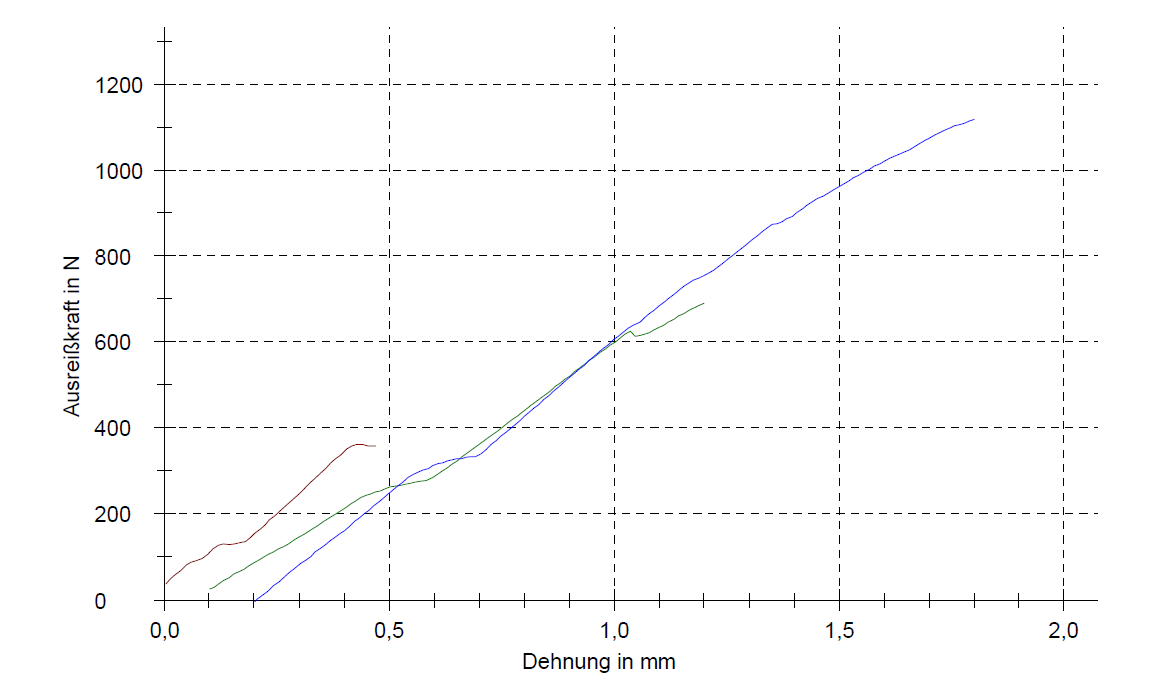
\includegraphics[width=\textwidth]{images/PA.png}
    \caption{PA: Zugkraft vs. Dehnung.}
\end{subfigure}
\hfill
\begin{subfigure}{0.45\textwidth}
    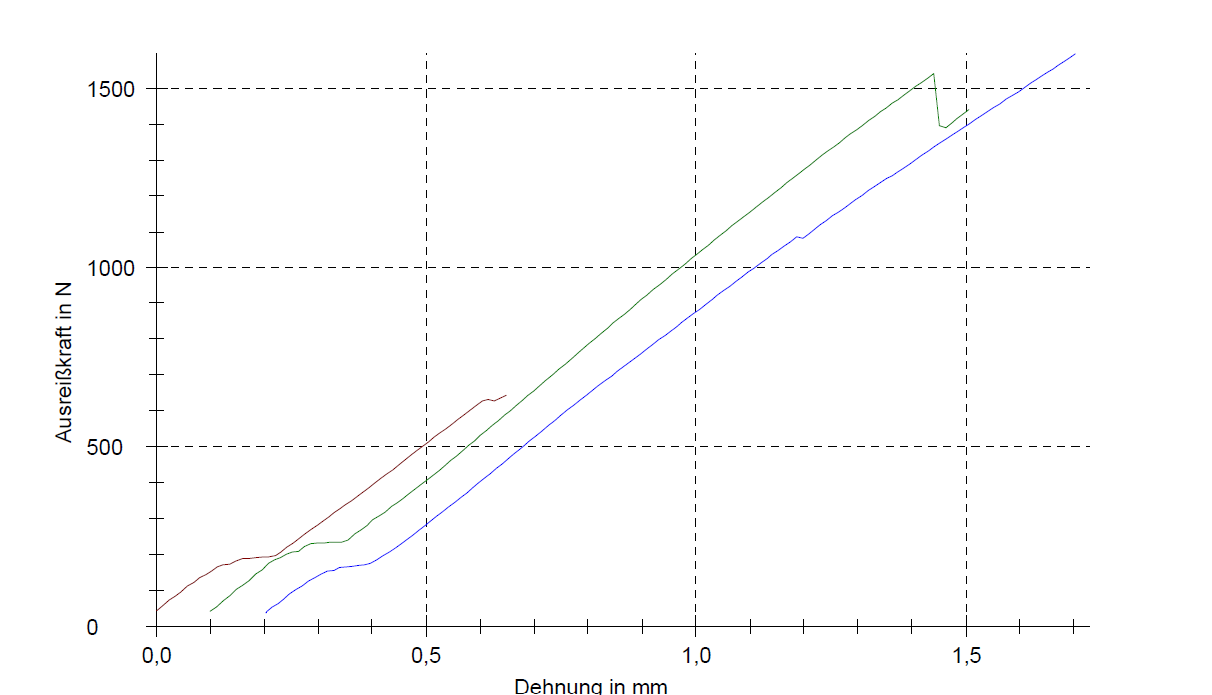
\includegraphics[width=\textwidth]{images/PC.png}
    \caption{PC: Zugkraft vs. Dehnung.}
\end{subfigure}
\\
\begin{subfigure}{0.45\textwidth}
    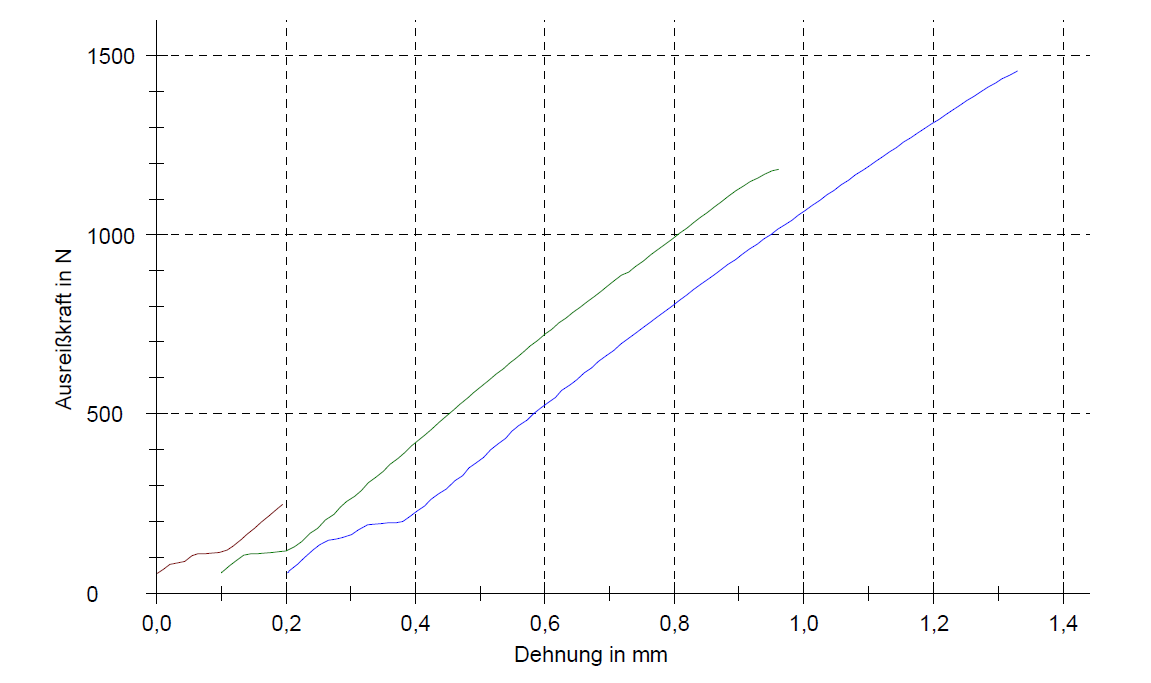
\includegraphics[width=\textwidth]{images/PMMA.png}
    \caption{PMMA: Zugkraft vs. Dehnung.}
\end{subfigure}
\hfill
\begin{subfigure}{0.45\textwidth}
    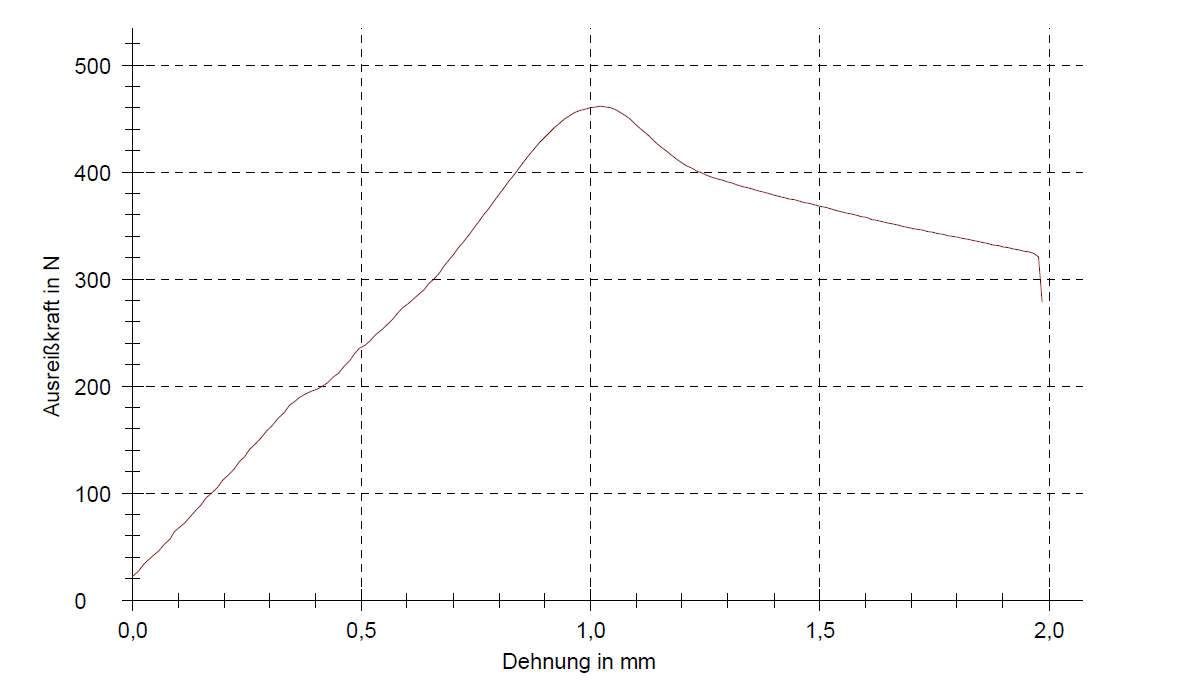
\includegraphics[width=\textwidth]{images/PP.png}
    \caption{PP: Zugkraft vs. Dehnung.}
\end{subfigure}
\caption{Vergleich der Zugkraft-Dehnungs-Kurven für verschiedene Materialien.}
\label{fig:load-strain}
\end{figure}

\renewcommand{\arraystretch}{1.1}
\setlength{\tabcolsep}{5pt}
\begin{table}[H]
\centering
\caption{Ergebnisse der Adh\"asionspr\"ufung}
\begin{tabular}{|p{2.5cm}|p{2.5cm}|p{3cm}|p{2.5cm}|p{4cm}|}
\hline
Material & Zustand & Fmax (N) Mittelwert & Verbesserung (\%) & Besonderheiten \\
\hline
PA & Unbehandelt & 722,89 & 54,7 & Gute Haftung, signifikante Verbesserung durch Oberflächenaktivierung. \\
   & Mit Plasmabehandlung (aktiviert)    & 1117,96 &       & \\
\hline
PP & Unbehandelt & 461,33 & 0     & Keine Verbesserung festgestellt. \\
   & Mit Plasmabehandlung (aktiviert)    & 461,33 &       & \\
\hline
PMMA & Unbehandelt & 961,66 & 51,4 & Starke Haftung bei aktivierter Oberfläche. \\
     & Mit Plasmabehandlung (aktiviert)    & 1456,1 &       & \\
\hline
PC & Unbehandelt & 1260,12 & 26,6 & Höchste Gesamtleistung. \\
   & Mit Plasmabehandlung (aktiviert)    & 1595,78 &       & \\
\hline
\end{tabular}
\label{tab:adhesion-results}
\end{table}

\section{Fazit}
Die Plasmabehandlung führte bei den meisten Materialien zu einer klaren 
Verbesserung der Haftung, insbesondere durch die Aktivierung der Oberfläche 
bei PA und PMMA. Diese Ergebnisse bestätigen die Effektivität der Methode zur 
Adhäsionsverbesserung. Zukünftige Untersuchungen sollten sich auf 
Materialien wie PP und die Optimierung des Klebeprozesses konzentrieren, 
um mögliche Fehler in der Klebstoffapplikation auszuschließen.

\section{Literaturverzeichnis}
\begin{thebibliography}{99}
    \bibitem{ref1} H. Hoffmann und J. Spindler, Verfahren in der Beschichtungs- und Oberfl"achentechnik, M"unchen: Carl Hanser Verlag GmbH \& Co. KG, 2020.
    \bibitem{ref2} D. Hegemann, H. Brunner, C. Oehr und D. Hegemann, "ScienceDirect," 2003. [Online]. Available: \url{https://www.sciencedirect.com/science/article/pii/S0168583X0300644X}. [Zugriff November 2024].
    \bibitem{ref3} V. Bucher und A. Kohler, "Praktikumsversuch Klebevorbehandlung mit Atmosph"arenplasma zur Vorlesung \"Beschichtungstechnologien\", WS2015/2016.
    \bibitem{ref4} W. Wei"sbach, Werkstoffkunde - Strukturen, Eigenschaften, Pr"ufung, Vieweg +Teubner Verlag, Springer Fachmedien Wiesbaden GmbH 2012, 2012.
    \bibitem{ref5} Monier, et al.: An investigation of adhesion mechanisms between plasma-treated PMMA support and aluminum thin films deposited by PVD. Applied Surface Science, 2021. HAL.
    \bibitem{ref6} Plasma-Technologie zur Rationalisierung von 2K-Prozessen. adh"asion KLEBEN \& DICHTEN, 2020. Springer Link.
\end{thebibliography}

\end{document}
